% TikZ Figures for CTUFT Main Paper
% Compile with: \usepackage{tikz,pgfplots}

%==============================================================================
% Figure 1: Reciprocal Internal Space Duality
%==============================================================================
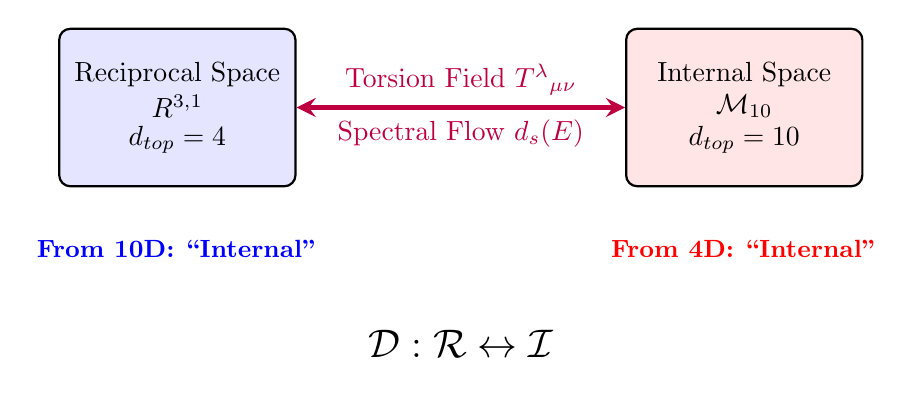
\begin{tikzpicture}[scale=1.2,
    box/.style={rectangle, draw, thick, minimum width=3cm, minimum height=2cm, rounded corners},
    arrow/.style={->, thick, >=stealth},
    label/.style={font=\small\bfseries}
]
    % 4D Reciprocal Space
    \node[box, fill=blue!10] (recip) at (0,0) {\shortstack{Reciprocal Space\\$\mathbb{R}^{3,1}$\\$d_{top} = 4$}};
    
    % 10D Internal Space
    \node[box, fill=red!10] (inter) at (6,0) {\shortstack{Internal Space\\$\mathcal{M}_{10}$\\$d_{top} = 10$}};
    
    % Torsion field coupling
    \draw[arrow, <->, line width=2pt, color=purple] (recip.east) -- (inter.west)
        node[midway, above] {Torsion Field $T^\lambda{}_{\mu\nu}$}
        node[midway, below] {Spectral Flow $d_s(E)$};
    
    % Perspective labels
    \node[label, blue] at (0,-1.5) {From 10D: ``Internal''};
    \node[label, red] at (6,-1.5) {From 4D: ``Internal''};
    
    % Duality symbol
    \node at (3,-2.5) {\Large$\mathcal{D}: \mathcal{R} \leftrightarrow \mathcal{I}$};
    
\end{tikzpicture}

%==============================================================================
% Figure 2: Spectral Dimension Flow
%==============================================================================
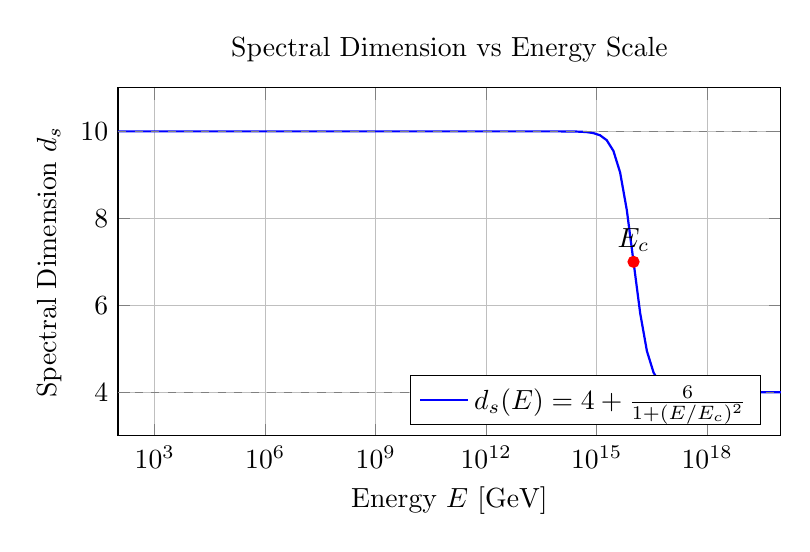
\begin{tikzpicture}[scale=1.0]
    \begin{axis}[
        width=10cm, height=6cm,
        xlabel={Energy $E$ [GeV]}, ylabel={Spectral Dimension $d_s$},
        xmin=1e2, xmax=1e20,
        ymin=3, ymax=11,
        xmode=log,
        grid=both,
        legend pos=south east,
        title={Spectral Dimension vs Energy Scale}
    ]
        % d_s = 4 + 6/(1+(E/E_c)^2)
        \addplot[domain=1e2:1e20, blue, thick, samples=100] 
            {4 + 6/(1+(x/1e16)^2)};
        \addlegendentry{$d_s(E) = 4 + \frac{6}{1+(E/E_c)^2}$}
        
        % Reference lines
        \addplot[dashed, gray] coordinates {(1e2,4) (1e20,4)};
        \addplot[dashed, gray] coordinates {(1e2,10) (1e20,10)};
        
        % E_c marker
        \addplot[only marks, mark=*, red] coordinates {(1e16,7)};
        \node at (axis cs:1e16,7.5) {$E_c$};
        
    \end{axis}
\end{tikzpicture}

%==============================================================================
% Figure 3: Energy Oscillation Interference
%==============================================================================
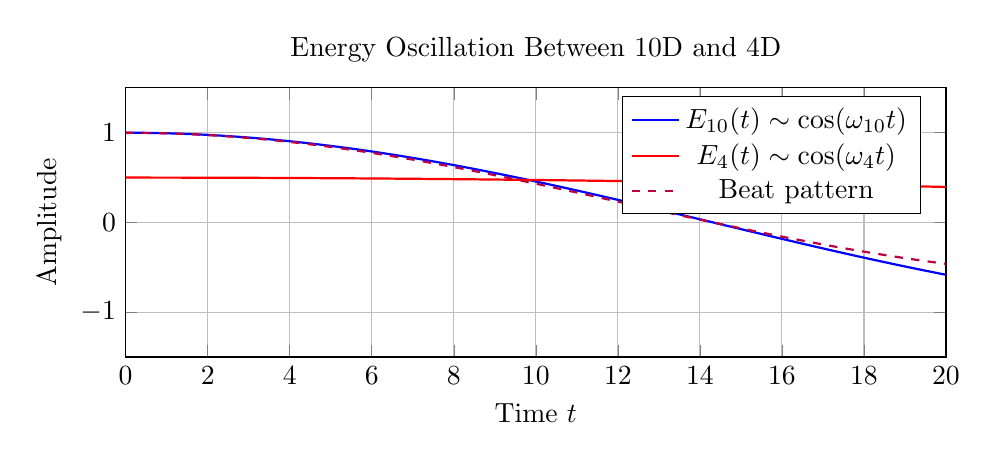
\begin{tikzpicture}[scale=1.0]
    \begin{axis}[
        width=12cm, height=5cm,
        xlabel={Time $t$}, ylabel={Amplitude},
        xmin=0, xmax=20,
        ymin=-1.5, ymax=1.5,
        grid=both,
        legend pos=north east,
        title={Energy Oscillation Between 10D and 4D}
    ]
        % E_10 mode
        \addplot[domain=0:20, blue, thick, samples=200] 
            {cos(2*pi*1.0*x)};
        \addlegendentry{$E_{10}(t) \sim \cos(\omega_{10}t)$}
        
        % E_4 mode
        \addplot[domain=0:20, red, thick, samples=200] 
            {0.5*cos(2*pi*0.3*x)};
        \addlegendentry{$E_4(t) \sim \cos(\omega_4t)$}
        
        % Beat frequency
        \addplot[domain=0:20, purple, thick, dashed, samples=200] 
            {cos(2*pi*1.0*x)*cos(2*pi*0.3*x)};
        \addlegendentry{Beat pattern}
        
    \end{axis}
\end{tikzpicture}

%==============================================================================
% Figure 4: CKM Matrix Comparison
%==============================================================================
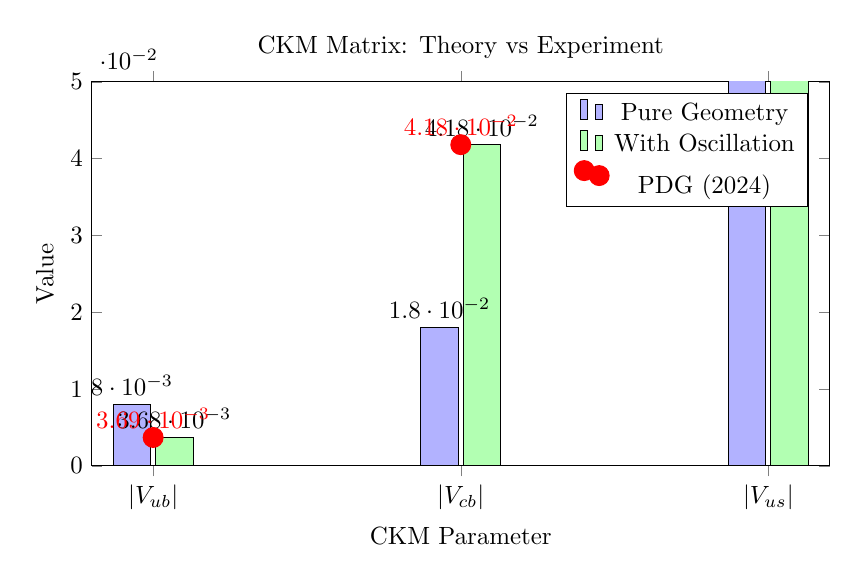
\begin{tikzpicture}[scale=0.9]
    % Bar chart comparing bare, corrected, and experimental values
    \begin{axis}[
        ybar,
        width=12cm, height=7cm,
        bar width=15pt,
        xlabel={CKM Parameter},
        ylabel={Value},
        ymin=0, ymax=0.05,
        xtick=data,
        symbolic x coords={$|V_{ub}|$, $|V_{cb}|$, $|V_{us}|$},
        legend pos=north east,
        nodes near coords,
        nodes near coords align={vertical},
        title={CKM Matrix: Theory vs Experiment}
    ]
        % Bare values
        \addplot[fill=blue!30] coordinates {
            ($|V_{ub}|$, 0.008)
            ($|V_{cb}|$, 0.018)
            ($|V_{us}|$, 0.200)
        };
        \addlegendentry{Pure Geometry}
        
        % Corrected values
        \addplot[fill=green!30] coordinates {
            ($|V_{ub}|$, 0.00368)
            ($|V_{cb}|$, 0.0418)
            ($|V_{us}|$, 0.236)
        };
        \addlegendentry{With Oscillation}
        
        % Experimental values
        \addplot[only marks, mark=*, mark size=4pt, red] coordinates {
            ($|V_{ub}|$, 0.00369)
            ($|V_{cb}|$, 0.04182)
            ($|V_{us}|$, 0.225)
        };
        \addlegendentry{PDG (2024)}
        
    \end{axis}
\end{tikzpicture}

%==============================================================================
% Figure 5: Six Gravitational Wave Polarizations
%==============================================================================
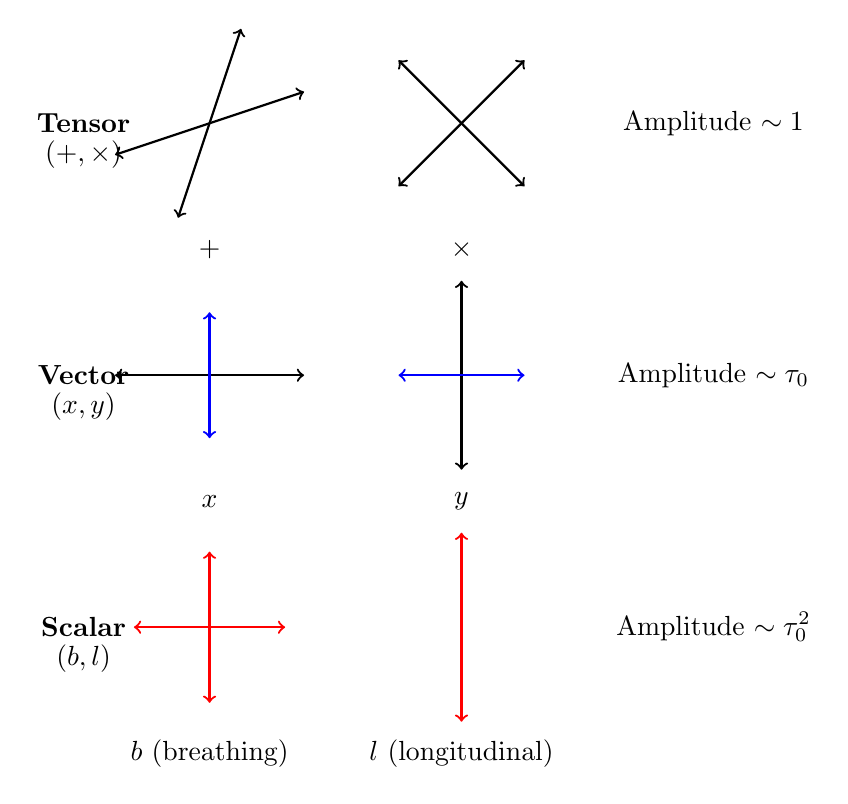
\begin{tikzpicture}[scale=0.8]
    % Tensor modes (+ and x)
    \begin{scope}[shift={(0,4)}]
        \node at (-2,0) {\textbf{Tensor}};
        \node at (-2,-0.5) {$(+, \times)$};
        
        % Plus polarization
        \draw[->, thick] (0,0) -- (1.5,0.5);
        \draw[->, thick] (0,0) -- (-1.5,-0.5);
        \draw[->, thick] (0,0) -- (0.5,1.5);
        \draw[->, thick] (0,0) -- (-0.5,-1.5);
        \node at (0,-2) {$+$};
        
        % Cross polarization
        \begin{scope}[shift={(4,0)}]
            \draw[->, thick] (0,0) -- (1,1);
            \draw[->, thick] (0,0) -- (-1,-1);
            \draw[->, thick] (0,0) -- (1,-1);
            \draw[->, thick] (0,0) -- (-1,1);
            \node at (0,-2) {$\times$};
        \end{scope}
    \end{scope}
    
    % Vector modes (x and y)
    \begin{scope}[shift={(0,0)}]
        \node at (-2,0) {\textbf{Vector}};
        \node at (-2,-0.5) {$(x, y)$};
        
        % x-mode
        \draw[->, thick] (0,0) -- (1.5,0);
        \draw[->, thick] (0,0) -- (-1.5,0);
        \draw[->, thick, blue] (0,0) -- (0,1);
        \draw[->, thick, blue] (0,0) -- (0,-1);
        \node at (0,-2) {$x$};
        
        % y-mode
        \begin{scope}[shift={(4,0)}]
            \draw[->, thick] (0,0) -- (0,1.5);
            \draw[->, thick] (0,0) -- (0,-1.5);
            \draw[->, thick, blue] (0,0) -- (1,0);
            \draw[->, thick, blue] (0,0) -- (-1,0);
            \node at (0,-2) {$y$};
        \end{scope}
    \end{scope}
    
    % Scalar modes (b and l)
    \begin{scope}[shift={(0,-4)}]
        \node at (-2,0) {\textbf{Scalar}};
        \node at (-2,-0.5) {$(b, l)$};
        
        % Breathing mode
        \draw[->, thick, red] (0,0) -- (1.2,0);
        \draw[->, thick, red] (0,0) -- (-1.2,0);
        \draw[->, thick, red] (0,0) -- (0,1.2);
        \draw[->, thick, red] (0,0) -- (0,-1.2);
        \node at (0,-2) {$b$ (breathing)};
        
        % Longitudinal mode
        \begin{scope}[shift={(4,0)}]
            \draw[->, thick, red] (0,0) -- (0,1.5);
            \draw[->, thick, red] (0,0) -- (0,-1.5);
            \node at (0,-2) {$l$ (longitudinal)};
        \end{scope}
    \end{scope}
    
    % Amplitude labels
    \node at (8,4) {Amplitude $\sim 1$};
    \node at (8,0) {Amplitude $\sim \tau_0$};
    \node at (8,-4) {Amplitude $\sim \tau_0^2$};
    
\end{tikzpicture}

%==============================================================================
% Figure 6: Cosmic Evolution with Spectral Dimension
%==============================================================================
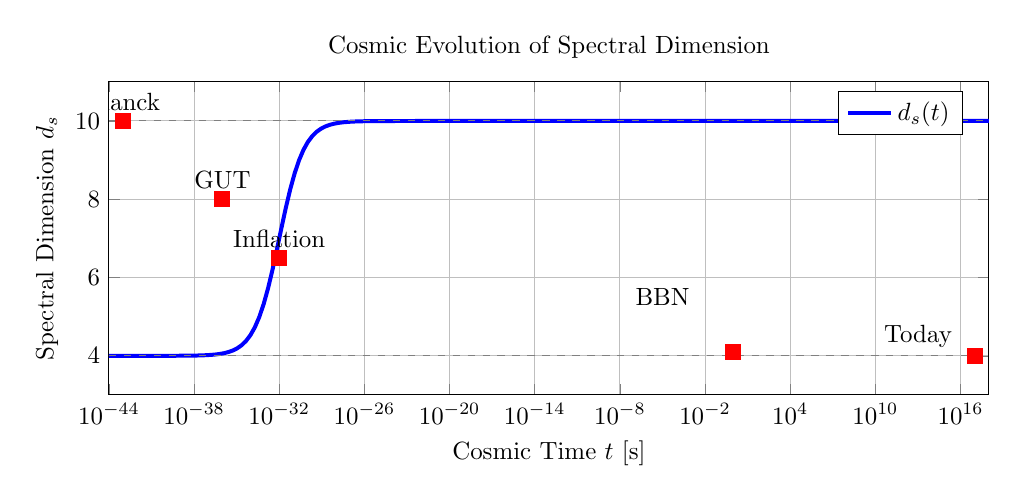
\begin{tikzpicture}[scale=0.9]
    \begin{axis}[
        width=14cm, height=6cm,
        xlabel={Cosmic Time $t$ [s]}, ylabel={Spectral Dimension $d_s$},
        xmin=1e-44, xmax=1e18,
        ymin=3, ymax=11,
        xmode=log,
        grid=both,
        legend pos=north east,
        title={Cosmic Evolution of Spectral Dimension}
    ]
        % Evolution curve
        \addplot[domain=1e-44:1e18, blue, ultra thick, samples=200] 
            {4 + 6/(1+(1e-32/x)^0.5)};
        \addlegendentry{$d_s(t)$}
        
        % Epoch markers
        \addplot[only marks, mark=square*, red, mark size=3pt] 
            coordinates {(1e-43,10) (1e-36,8) (1e-32,6.5) (1e0,4.1) (1e17,4)};
        
        % Labels
        \node at (axis cs:1e-43,10.5) {Planck};
        \node at (axis cs:1e-36,8.5) {GUT};
        \node at (axis cs:1e-32,7) {Inflation};
        \node at (axis cs:1e-5,5.5) {BBN};
        \node at (axis cs:1e13,4.5) {Today};
        
        % Reference lines
        \addplot[dashed, gray] coordinates {(1e-44,4) (1e18,4)};
        \addplot[dashed, gray] coordinates {(1e-44,10) (1e18,10)};
        
    \end{axis}
\end{tikzpicture}

%==============================================================================
% Figure 7: Interference Factor vs Phase Difference
%==============================================================================
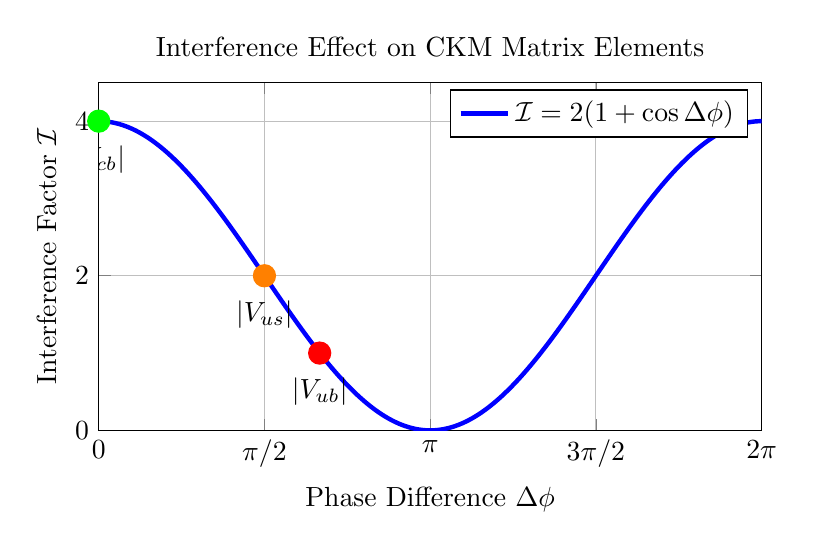
\begin{tikzpicture}[scale=1.0]
    \begin{axis}[
        width=10cm, height=6cm,
        xlabel={Phase Difference $\Delta\phi$}, ylabel={Interference Factor $\mathcal{I}$},
        xmin=0, xmax=360,
        ymin=0, ymax=4.5,
        xtick={0,90,180,270,360},
        xticklabels={$0$,$\pi/2$,$\pi$,$3\pi/2$,$2\pi$},
        grid=both,
        title={Interference Effect on CKM Matrix Elements}
    ]
        % I = 2(1 + cos(delta_phi))
        \addplot[domain=0:360, blue, ultra thick, samples=200] 
            {2*(1+cos(x))};
        \addlegendentry{$\mathcal{I} = 2(1+\cos\Delta\phi)$}
        
        % Mark V_ub (suppression)
        \addplot[only marks, mark=*, red, mark size=4pt] 
            coordinates {(120,1)};
        \node at (axis cs:120,0.5) {$|V_{ub}|$};
        
        % Mark V_cb (amplification)
        \addplot[only marks, mark=*, green, mark size=4pt] 
            coordinates {(0,4)};
        \node at (axis cs:0,3.5) {$|V_{cb}|$};
        
        % Mark V_us (neutral)
        \addplot[only marks, mark=*, orange, mark size=4pt] 
            coordinates {(90,2)};
        \node at (axis cs:90,1.5) {$|V_{us}|$};
        
    \end{axis}
\end{tikzpicture}

% End of figures